% !TEX program = xelatex
\def\thelstlisting{}

%不需要区分奇偶页的请使用下面一行
\documentclass[a4paper,AutoFakeBold,oneside,12pt]{book}
%需要区分奇偶页的(即每一章第一页一定在奇数页上)请使用下面一行
%\documentclass[a4paper,AutoFakeBold,openright,12pt]{book}
\usepackage{BUPTthesisbachelor}
\usepackage{setspace}

%\lstdefinestyle{sharpc}{language=[Sharp]C, frame=lrtb, rulecolor=\color{blue!80!black}}


%%%%%%%%%%%%%%%%%%%%%%%%% Begin Documents %%%%%%%%%%%%%%%%%%%%%%%%%%
\begin{document}

% 封面
%\blankmatter
%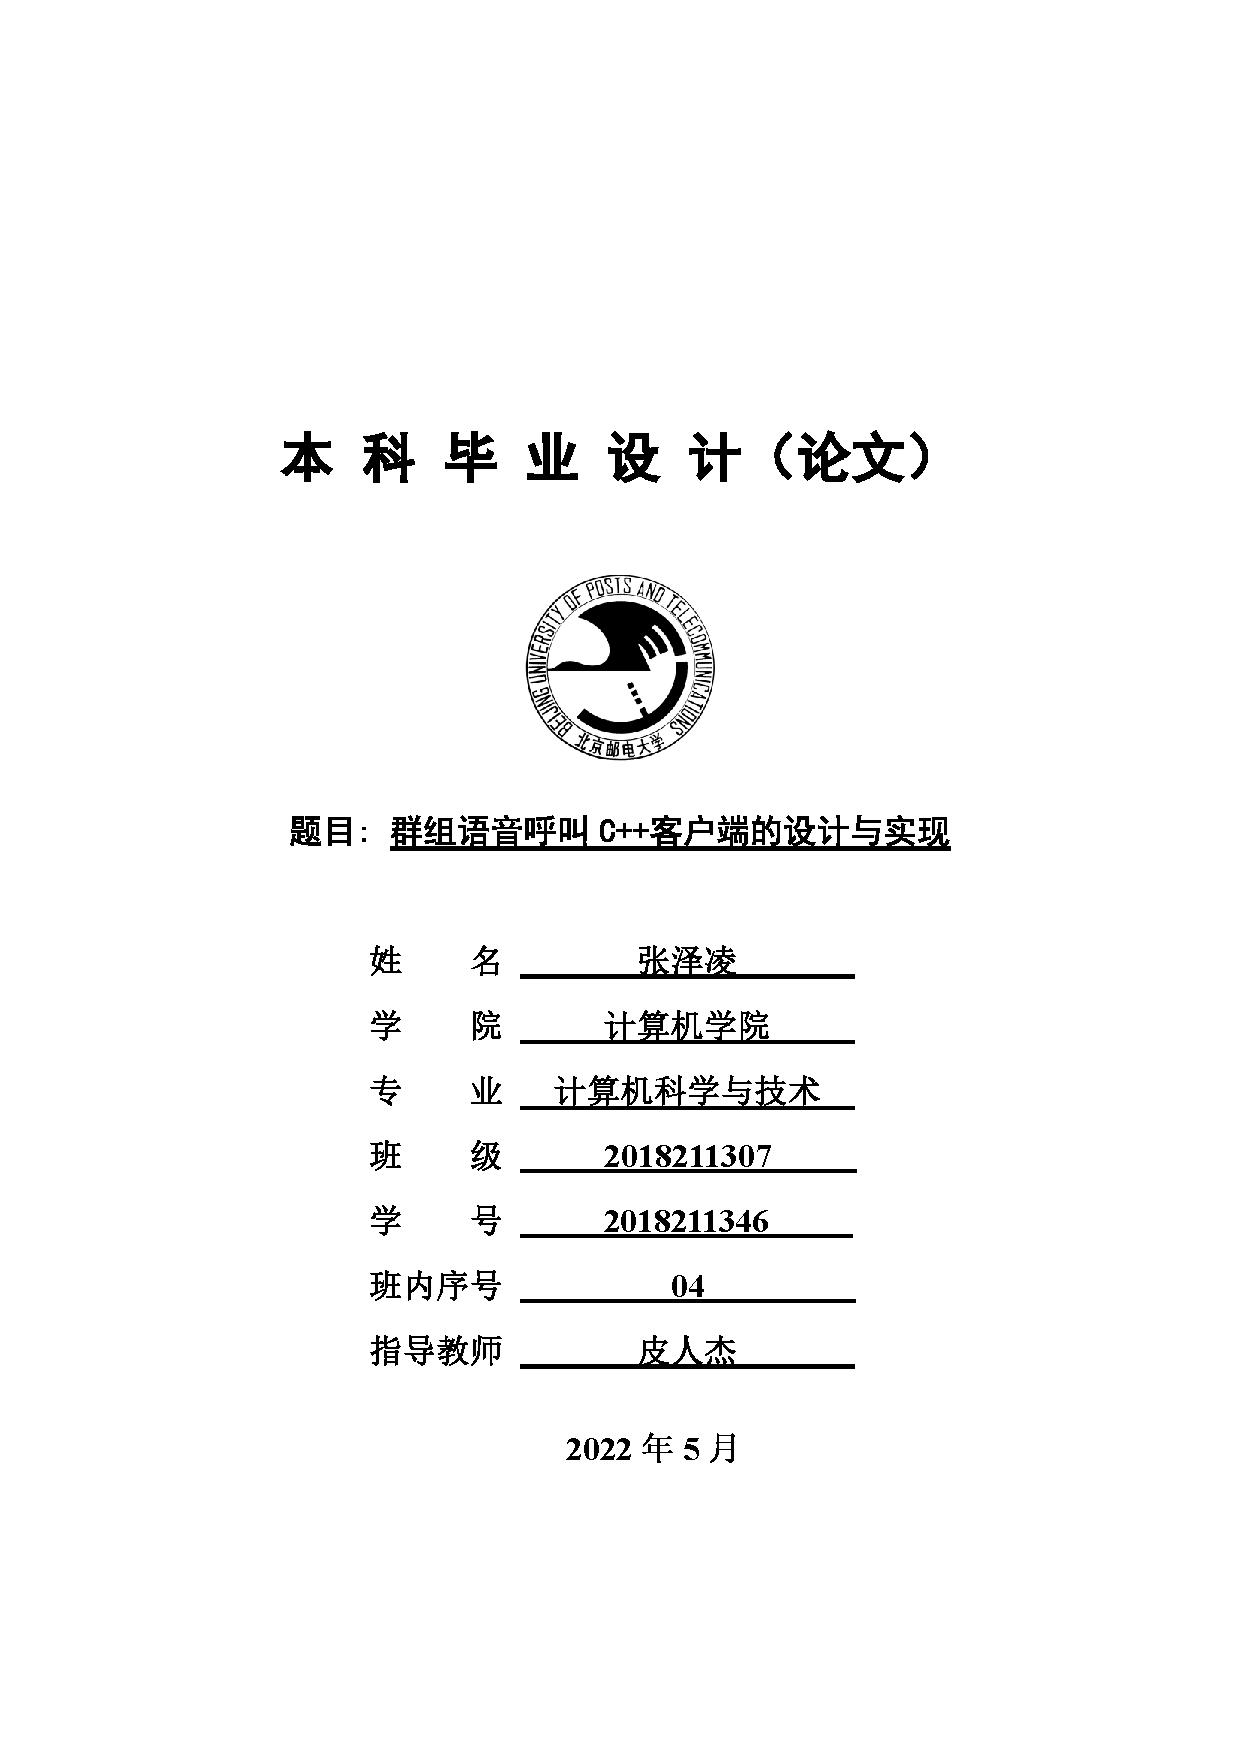
\includepdf[pages=-]{docs/cover.pdf}  

% 任务书
%\blankmatter
%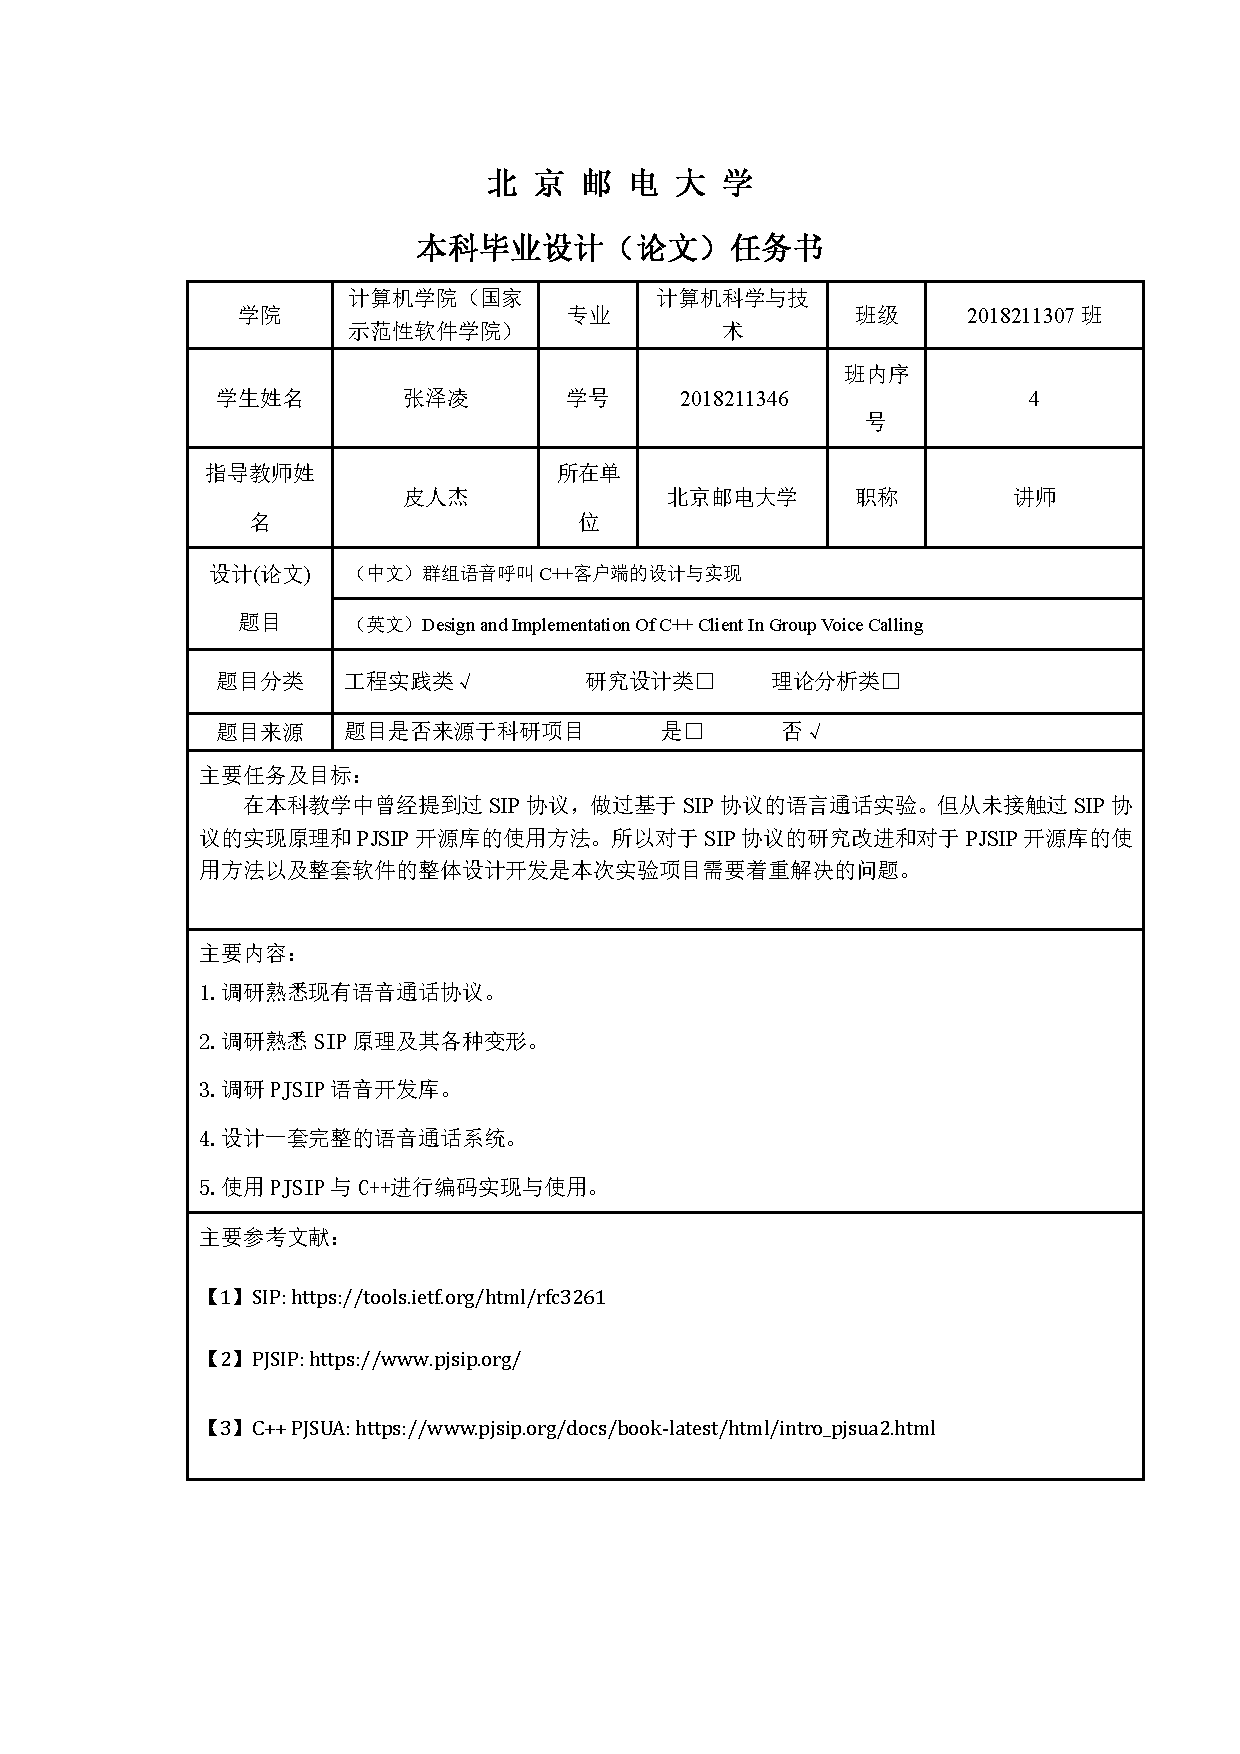
\includepdf[pages=-]{docs/task.pdf}  

% 成绩评定表
%\blankmatter
%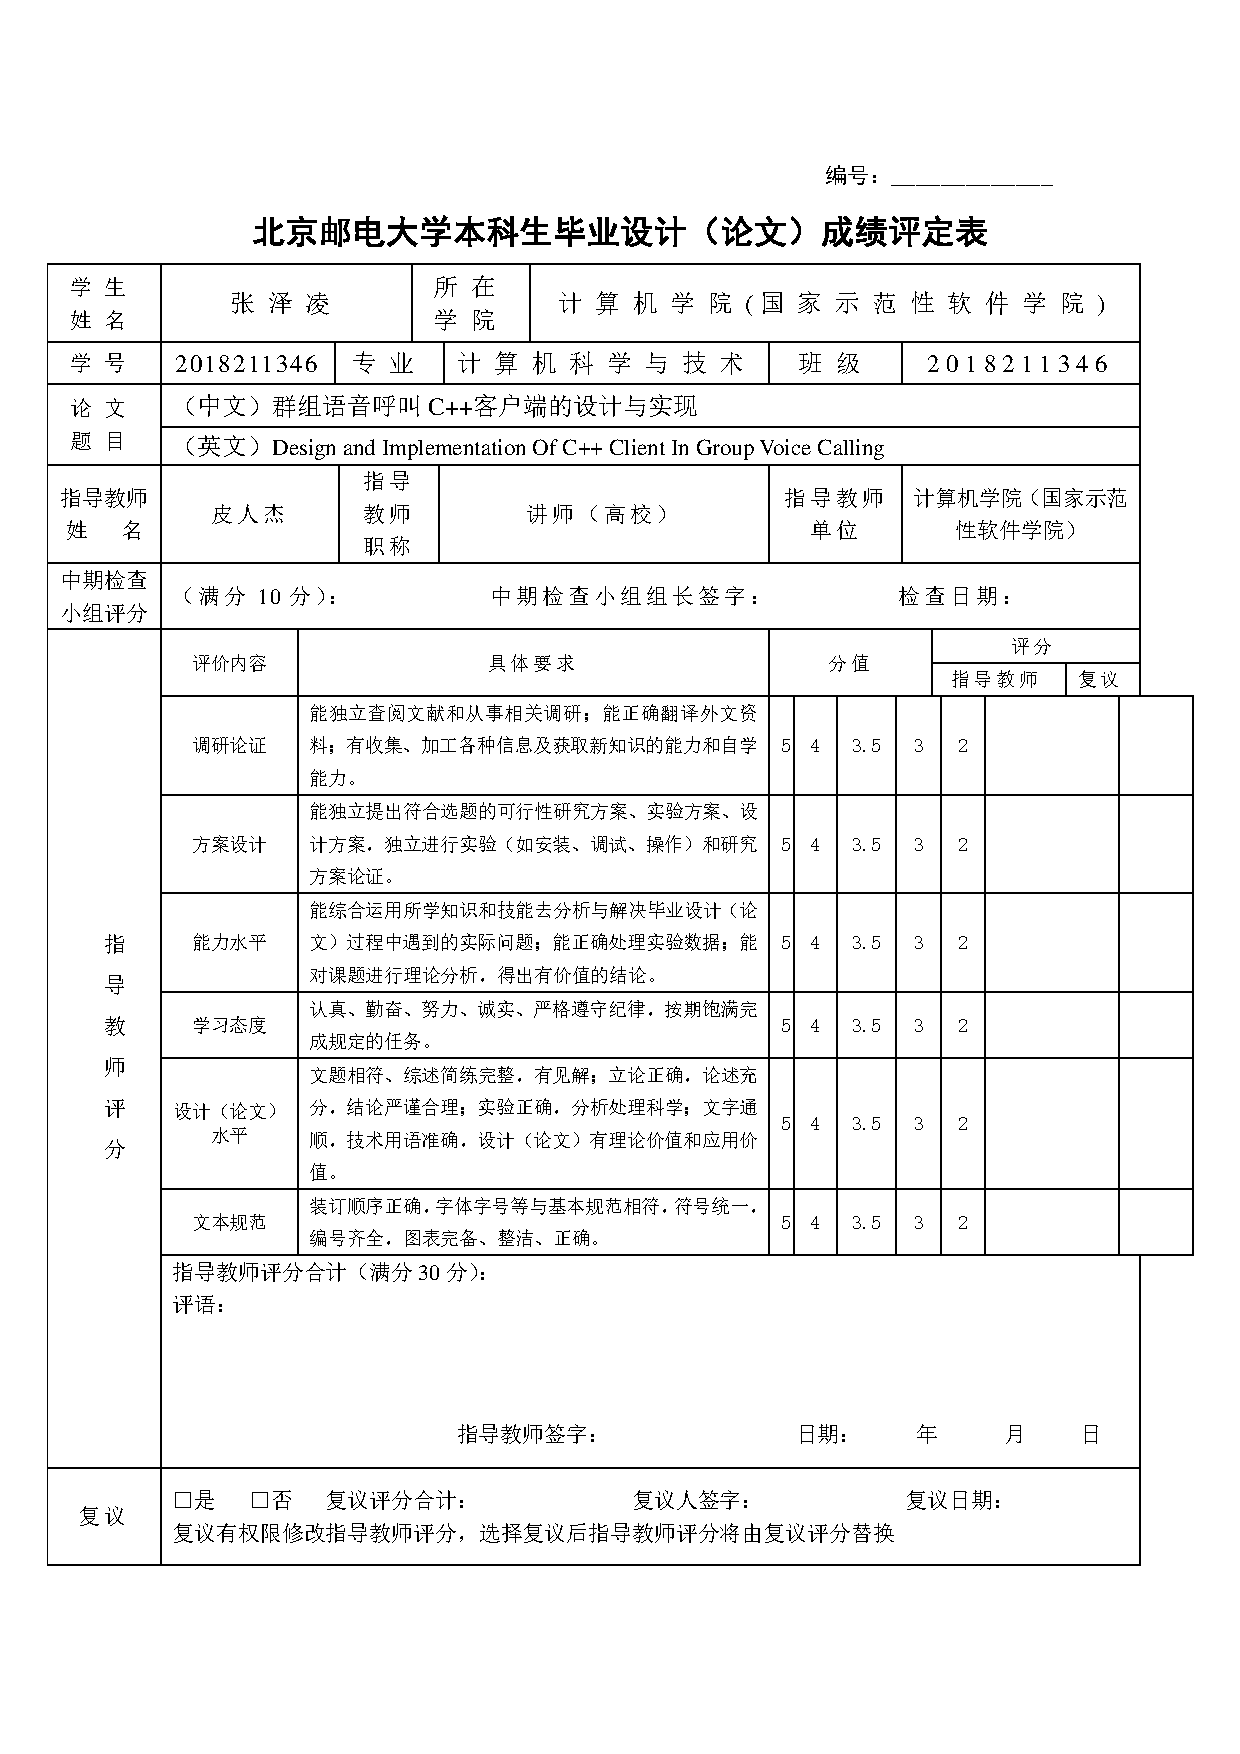
\includepdf[pages=-]{docs/scoreTable.pdf}  

% 诚信声明
%\blankmatter
%
\includepdf[pages=-]{docs/statement.pdf} 

%%%%%%%%%%%%%%%%%%%%%%%%%%%%%%%%%%%%%%%%%%%%%%%%%%%%%%%%%%%%%%%%%%%%
%                                                                  %
%   Copyright (c) 2010 - 2011 Caspar Zhang <casparant@gmail.com>   %
%                                                                  %
%   This copyrighted material is made available to anyone wishing  %
%   to use, modify, copy, or redistribute it subject to the terms  %
%   and conditions of the GNU General Public License version 2.    %
%                                                                  %
%   This program is distributed in the hope that it will be        %
%   useful, but WITHOUT ANY WARRANTY; without even the implied     %
%   warranty of MERCHANTABILITY or FITNESS FOR A PARTICULAR        %
%   PURPOSE. See the GNU General Public License for more details.  %
%                                                                  %
%   You should have received a copy of the GNU General Public      %
%   License along with this program; if not, write to the Free     %
%   Software Foundation, Inc., 51 Franklin Street, Fifth Floor,    %
%   Boston, MA 02110-1301, USA.                                    %
%                                                                  %
%%%%%%%%%%%%%%%%%%%%%%%%%%%%%%%%%%%%%%%%%%%%%%%%%%%%%%%%%%%%%%%%%%%%

% 你只需要修改下面几行就可以完成大部分内容的填写,
% 这要求你具有一定的LaTeX基础,但是如果你足够聪明,
% 不具有LaTeX基础也可以完成。

% 论文中文题目
\def\thesistitle{群组语音呼叫C++客户端的设计与实现}

% 论文英文题目
%提示:英文摘要页的标题注意格式要求。
\def\thesistitleen{Design and Implementation Of C++ Client In Group Voice Calling}

% Thank Words
\def\thankwords{

此处请写致谢的内容。

它可以有多段。
}
    % Main items 
% !TEX program = xelatex
%%%%%%%%%%%%%%%%%%%%%%%%%%%%%%%%%%%%%%%%%%%%%%%%%%%%%%%%%%%%%%%%%%%%
%                                                                  %
%   Modified by Bing Hsu <hello@antinucleon.com> 2013              %
%   Forked From (c) 2010 - 2011 Caspar Zhang <casparant@gmail.com> %
%                                                                  %
%   This copyrighted material is made available to anyone wishing  %
%   to use, modify, copy, or redistribute it subject to the terms  %
%   and conditions of the GNU General Public License version 2.    %
%                                                                  %
%   This program is distributed in the hope that it will be        %
%   useful, but WITHOUT ANY WARRANTY; without even the implied     %
%   warranty of MERCHANTABILITY or FITNESS FOR A PARTICULAR        %
%   PURPOSE. See the GNU General Public License for more details.  %
%                                                                  %
%   You should have received a copy of the GNU General Public      %
%   License along with this program; if not, write to the Free     %
%   Software Foundation, Inc., 51 Franklin Street, Fifth Floor,    %
%   Boston, MA 02110-1301, USA.                                    %
%                                                                  %
%%%%%%%%%%%%%%%%%%%%%%%%%%%%%%%%%%%%%%%%%%%%%%%%%%%%%%%%%%%%%%%%%%%%

%%%%%%%%%%%%%%%%%%%%%%%%%%%%%%%%%%%%%%%%%%%%%%%%%%%%%%%%%%%%%%%%%%%%
%                                                                  %
%   Copyright (c) 2010 - 2011 Caspar Zhang <casparant@gmail.com>   %
%                                                                  %
%   This copyrighted material is made available to anyone wishing  %
%   to use, modify, copy, or redistribute it subject to the terms  %
%   and conditions of the GNU General Public License version 2.    %
%                                                                  %
%   This program is distributed in the hope that it will be        %
%   useful, but WITHOUT ANY WARRANTY; without even the implied     %
%   warranty of MERCHANTABILITY or FITNESS FOR A PARTICULAR        %
%   PURPOSE. See the GNU General Public License for more details.  %
%                                                                  %
%   You should have received a copy of the GNU General Public      %
%   License along with this program; if not, write to the Free     %
%   Software Foundation, Inc., 51 Franklin Street, Fifth Floor,    %
%   Boston, MA 02110-1301, USA.                                    %
%                                                                  %
%%%%%%%%%%%%%%%%%%%%%%%%%%%%%%%%%%%%%%%%%%%%%%%%%%%%%%%%%%%%%%%%%%%%

% 你只需要修改下面内容就可以完成中英文摘要,
% 这要求你具有一定的LaTeX基础,但是还是那句话,
% 如果你足够聪明,不具有LaTeX基础也可以完成。

% 中文摘要
\def\abstractzh{
语音通信在后疫情时代已成为人们不可或缺的交流手段,作为传统手机通讯的迭代升级,承载于网络的语音通信VOIP技术,在拥有不输于传统通话的实时性的基础上更加强化了方便性与灵活性。
因此,VOIP技术不止能做到传统手机通讯的点对点模式,还能方便地模拟出譬如多人会议室等多对多的群组聊天场景并加以管理。更进一步,只要该设备支持某种特定协议,该设备甚至可以不局限于手机,
能实现电话、电脑、传真机、网页等多平台相互通信,从而大大提高跨平台的能力。

为了研究VOIP技术,本论文将会从SIP协议,一个在VOIP技术中广泛运用的协议入手。利用PJSIP开发库,设计并实现一个群组语音呼叫客户端及其配套服务器。
该系统的主要功能是实现客户端之间的群组语音通话和群组的管理。最终为用户提供一个交互友好、使用方便、效率和质量高的群组语音通信系统。
}

% 中文关键字 
% TODO: 改成可变长度的
\def\abszhkeyone{VOIP}
\def\abszhkeytwo{SIP}
\def\abszhkeythree{PJSIP}
\def\abszhkeyfour{语音通信}
\def\abszhkeyfive{群组管理}

% ABSTRACT
\def\abstracten{
%Your abstract here, to make a new paragraph, give an extra blank line please.
Voice communication has become an indispensable means of communication in the post epidemic era. 
As an iterative upgrade of traditional mobile communication, VoIP technology, which is carried on the network, 
has strengthened the convenience and flexibility on the basis of the real-time performance of traditional calls. 
Therefore, VoIP technology can not only achieve the point-to-point mode of traditional mobile communication, 
but also easily simulate and manage many to many group chat scenes such as multi person conference room. 
Further, as long as the device supports a specific protocol, the device can even be not limited to mobile phones, 
and can realize multi platform communication such as telephone, computer, fax machine and web page, 
so as to greatly improve the cross platform ability.

In order to study VoIP technology, this paper will start with SIP protocol, a protocol widely used in VoIP technology. 
Using pjsip development library, a group voice call client and its supporting server are designed and implemented. 
The main function of the system is to realize group voice call and group management between clients. 
Finally, it provides users with a group voice communication system with friendly interaction, convenient use, high efficiency and high quality.
%Abstract done
}

% Key Words 
% TODO: 改成可变长度的
\def\absenkeyone{VOIP}
\def\absenkeytwo{SIP}
\def\absenkeythree{PJSIP}
\def\absenkeyfour{Voice Communication}
\def\absenkeyfive{Group Management}




% 中文摘要
\begin{titlepage}

    \pagestyle{empty}

    \begin{spacing}{1.05}
        \centering
        % 如果你的标题太长,可能会换行;如果你对换行位置不满意,请调节下面第一个{}的参数
        \parbox[c]{.75\textwidth}{\thesistitlefont{\thesistitle}}
    \end{spacing}

    \begin{spacing}{1.5}
        \centering
        \sanhao\quad{} \\ 
        \abszhname{摘\quad{}要} \\ 
    \end{spacing}
    \xiaosanhao\quad{}

    \normalsize

    \abstractzh
    

    \quad{}

    \par\noindent\abszhkey{关键词}\quad{}%
    \abszhkeys{\abszhkeyone\quad{}%
                      \abszhkeytwo\quad{}%
                      \abszhkeythree\quad{}%
                      \abszhkeyfour\quad{}%
                      \abszhkeyfive}%
\end{titlepage}

\thispagestyle{empty}

% Abstract
\begin{titlepage}

    \pagestyle{empty}

    \begin{spacing}{1.05}
        \centering
        % 如果你的标题太长,可能会换行;如果你对换行位置不满意,请调节下面第一个{}的参数
        \parbox[c]{.70\textwidth}{\thesistitleenfont{\thesistitleen}}
    \end{spacing}

    \begin{spacing}{1.5}
        \centering
        \sanhao\quad{} \\ 
        \abszhname{ABSTRACT} \\ 
    \end{spacing}
    \xiaosanhao\quad{}
    \normalsize

    \abstracten
    
    \quad{}

    \par\noindent\absenkey{KEY WORDS}\quad{}%
    \absenkeys{\absenkeyone\quad{}%
                      \absenkeytwo\quad{}%
                      \absenkeythree\quad{}%
                      \absenkeyfour\quad{}%
                      \absenkeyfive}%
\end{titlepage}

\thispagestyle{empty}  % Abstract
\fancypagestyle{plain}{\pagestyle{frontmatter}}
\frontmatter\tableofcontents % Content


% 正文
\newpage\mainmatter
\fancypagestyle{plain}{\pagestyle{mainmatter}}
%\let\cleardoublepagebak=\cleardoublepage
%\let\cleardoublepage\relax % Make new chapter stay on old page

%%%%%%%%%%%%%%%%%%%%%%%%%%%%% Main Area %%%%%%%%%%%%%%%%%%%%%%%%%%%%

\chapter{引言}
\section{课题背景}
在语音通信已经长足发展的今天,微信、QQ、飞书等软件所提供的文字聊天以及音视频通话功能已经成为我们生活中不可替代的一部分。作为传统电话通信和面对面会议的迭代升级版,
通过网络进行的音视频通信能充分发挥网络本身的即时性,方便性,灵活性等。同理,网络会议也能轻松完成传统会议室会议无法做到的巨大容量和极其方便的群组管理,通过简单的手指点击
即可加入、管理、退出来自全国各地千百公里外的人们共同参加的会议,省时省力又省心。
特别是新冠疫情爆发以来,国内的疫情管理政策与被感染的风险使得人们不惜跨省出差只为参加某个重要的会议成为了过去式,
人们对于通过网络进行无接触交流互动的需求大幅增加。而语音通信在某种程度上相比传统文字聊天更加方便快捷,在传统文字聊天的实时性基础上可以传递大容量大信息量的语音信息,
在当前的快节奏生活时代显然更加适用。因此,在此大背景下,本课题将通过利用SIP协议与开源的PJSIP语音开发库自行设计并编码实现一套完整的聊天通话功能软件,
探讨如何构建简单易用的语音通信客户端,以及如何使用语音通信进行无接触交流。提升对语音通话领域发展的理解与认识,并尝试在生活中为我们提供一定的便利。
\section{课题任务}
该毕业设计的总体目标是设计并实现一个群组语音通话客户端。
\subsection{课题内容}
而具体研究实现的部分是基于SIP协议的语言通话群组切换功能的实现。
计划使用由C语言编写的开源PJSIP协议库进行开发,配合C++/QT进行可视化操作的编写。
最终完成的结果将为一个工作在同一个网络域下的非代理的,带图形界面的PC端群组语言通话客户端及其配套的服务器。
\subsection{本人承担任务}
本人承担除提出该课题任务之外的全部工作,包括:论文文献阅读、相关技术学习、软件需求分析、软件模块分析、软件编码实现以及论文撰写。
\newpage
\section{论文结构}
本论文结构借鉴于《软件工程》教材中的软件开发步骤,并以此作为模板进行章节划分,具体的划分如下:

第一章:引言;

第二章:相关技术的介绍;

第三章:系统的需求分析;

第四章:系统的总体设计;

第五章:系统主要功能模块的详细设计与实现;

第六章:系统测试;

第七章:结束语;
\chapter{相关技术介绍}
\section{VoIP}
\subsection{VoIP简介}
VoIP全称Voice over Internet Protocol,即基于网络协议(又称IP协议)的语音通话。是一种利用网络来开展语音通话或者多媒体会议的技术手段,即通过互联网来进行通信。
VoIP又被称为IP电话、互联网电话、宽带电话或宽带电话服务等,与SIP协议有着密不可分的关系。VoIP技术协议栈大致包括了音视频编解码协议、连接控制协议和传输协议等。
VoIP技术可使在各种终端设备接入互联网,包括VoIP电话、PC个人电脑和智能手机等,能通过移动网络、Wi-Fi网络进行短信发送以及语音多媒体通话,
并且能够支持跨网络、跨地区甚至跨国等多种通信场景。本论文所尝试实现的语音通话功能即可称之为VoIP技术。
\subsection{VoIP原理}
VoIP的基本原理是利用通过在设备终端上对语音信息进行采样,将采样后的语音数据编码为数字数据并使用压缩算法进行压缩,再通过网络建立IP连接,传输层可以采用TCP也可以采用UDP,
这取决于当前VoIP业务所传输的数据对象和QoS通话质量要求。通过IP网络将数据报发送到目的终端后,再进过上述步骤的反向操作,即解压缩、拼接、解码,最终通过扬声器播放出来,
从而达到使用互联网进行语言通话的目的。

IP网关不仅是VoIP技术的关键,也是VoIP网络搭建中的核心设备。它能对各个地区电话号码的区号进行映射,并转换为相应地区的IP网关地址。
这些映射信息都存放在一个数据库中,该数据库将配合VoIP软件完成呼叫与接听、数字语音编码与IP数据报的构建组装、路由管理等功能。

在用户通过网络拨打长途VoIP电话时,用户所在地区的IP网关会根据数据库中的电话区号资料来确定目的IP地址,完成地区电话号码到目的IP地址的映射转换,
并以此地址为目的地址构造IP数据报,同时根据IP网关中存放的路由表做出最佳路由选择以减少传输时延。
在一些Internet网络尚未接入或者暂时未设置默认IP网关的地区,也可以灵活地手动设置路由选项,从离该地区最近的可用IP网关建立传统电话网转接,仍可以实现通信。
\subsection{VoIP常用控制协议}
在VoIP技术中,除开设备对模拟信号语音的采样协议、对数字语音的编码解码协议以外,最重要的就是终端与终端之间建立连接时所用的控制协议。
这些控制协议规定了终端之间的连接状态、连接数、通话类型、会议类型、采用的编解码协议等需要双方共同商讨有关连接的问题。

VoIP技术中常用的控制协议有H.323、SIP、MEGACO和MGCP等协议。
\subsubsection{H.323}
H.323是一个ITU-T国际电信联盟电信标准分局所定义的协议,该协议最开始用于管理控制LAN局域网上的多媒体会议。后来随着技术的发展,
在H.323协议的第二个版本中,对当时的互联网新业务尤其是多媒体通信方面进行了扩展,从功能上支持了互联网的电话业务,使VoIP技术在H.323协议的控制下成为可能。
该协议既支持点对点通信,也支持多点通信。H.323协议定义了四种基本逻辑组成部分:终端、网关、关守和MCU多点控制单元。其中终端、网关和MCU多点控制单元均被视为终端点。

H.323协议是一个框架协议,是一系列用于实现基于IP网络提供音视频和数据实时传送功能的协议整合。
H.323协议组中两个最重要的,也是在软件开发过程中一般需要程序员自己根据协议内容流程进行实现的协议分别是RTP实时传输协议和RTCP实时控制协议。

H.323协议中规定音频流和视频流分组在编码后必须使用RTP实时传输协议进行封装,并通过两个相互传输数据的音视频终端所组成的一个UDP Socket进行承载。
而实时控制协议RTCP用来评估所有的会话和QoS连接质量,并根实时根据连接的情况或服务器会话管理做出的动作,在各个通信方终端之间提供反馈信息。
其对应的控制数据以及其他功能性的的分组都通过TCP或UDP进行操作,这取决于当前业务的通话质量要求或者当前的网络状态。
H.323协议还规定,所有运行H.323协议的终端都必须有一个语音编码器,可选一个视频编码器,其中语音编码器的编码协议要求最低必须支持G.711标准。
\subsubsection{SIP}
SIP会话发起协议是VoIP技术最常用的协议,是建立VOIP连接的IETF标准。SIP是一种应用层控制协议,一个基于UDP的应用层信令控制协议,用于创建、管理和释放会话。
SIP协议结构与HTTP协议的结构相似,其过程都是客户端向服务器发出请求,服务器收到请求并处理这些请求后给客户端返回客户端所请求的响应。
一次请求和响应组成SIP协议中的一次事务。

SIP协议即是本论文中用于实现VoIP功能所用到的的会话管理协议,关于SIP协议本身的协议结构将会在下一个小节进行详细介绍。
\subsubsection{MGCP}
MGCP媒体网关控制协议定义了呼叫控制单元,即呼叫代理或媒体网关与电话网关之间的通信服务。MGCP是一种控制协议,该协议允许中央控制台监测所有的网关和IP电话事件,
并通知它们向指定地址发送内容。在MGCP结构中,网关外部存在智能呼叫控制,并由呼叫控制单元,即呼叫代理来处理。
同时,呼叫控制单元之间保持互相同步,向网关发送一致的命令,以便网关可以按照正确无误的命令来处理呼叫。
\subsubsection{MEGACO/H.248}
Megaco/H.248是一种用于控制在物理上相互分隔的多媒体网关协议单元的协议,因此可以做到从媒体转换中将呼叫控制的单元分离出去。
Megaco媒体网关控制协议是IETF和ITU-TH.248建议共同努力的结果。
Megaco/H.248阐明了用于将交换电路语言转换到基于IP数据报的流量通信的MG媒体网关和规定服务于这种流量的服务逻辑所定义的媒介网关控制器之间的关系。
Megaco/H.248中的通知媒体网关将单元数据流或数据包中填充来自于数据包或单元数据网络之外的数据流,比如在RTP实时传输协议中产生的数据流量。

从VoIP功能结构和网关控制协议的关系这方面来看,Megaco/H.248与MGCP在本质上几乎完全相同,只是Megaco/H.248相比于MGCP能支持更多样更广泛的网络,如ATM网络等。
\section{SIP协议}
\subsection{SIP协议简介}
SIP 协议全称为Session Initiation Protocol,即会话发起协议,是一个基于UDP的应用层信令控制协议。用于创建、管理和释放会话。这些会话可以是多种多样的不同应用,
比如Internet多媒体会议、IP电话或是其他各种多媒体应用。参与会话的终端可以通过组播或者网状单播亦或是这两者的组合进行通信。
随着计算机科学技术的进步以及互联网的普及和网络应用发展,便捷、廉价的IP数据网络采用新式的分组交换技术,渐渐取代了基于电路交换的传统电话网在通信领域的核心地位。
SIP协议是一个会话管理协议,这意味着它的一个重要的特点是SIP协议只需要声明如何对会话进行创建、管理和释放等操作,而不需要对会话本身的操作方式进行定义,
也不需要对承载对话的网络有所限制。这种强大的灵活性意味着SIP协议可以用于各种各样的应用,比如Internet多媒体会议、IP电话或是其他各种多媒体应用。
SIP协议规定SIP控制消息本身是基于文本的,对开发人员具有很好的可阅读性和可调试性,使构建新服务的编程工作更加简便。
和邮件协议SMTP相同,SIP协议同样基于MIME类型描述进行了重用,使得由SIP协议管理会话的应用软件可以自动启动运行。
\subsection{SIP协议栈}
在协议栈方面,SIP协议组合重用了几个当下已经成熟的协议。

在网络层方面,由于SIP协议是应用层协议,独立于网络层,在网络层采用TCP/IP协议。%网络层采用TCP/IP协议
在此层之下的数据链路层和物理层可以使用任意支持IP协议的数据链路和物理网络,比如可以是采用ATM网络的IP,也可以是承载于PPP协议之上的IP。

在传输层方面,SIP协议与一般协议不同,开发者可以根据当前网络状态和所开发的服务要满足的要求,对传输层协议进行自由选择。
如果项目要求低时延、低带宽、低资源消耗,且需要实现SIP快速连接,则可以考虑采用UDP协议。但是UDP是一个无连接的协议,且不保证可靠性,因此在UDP上进行SIP协议控制存在不安全性。
而TCP协议对SIP报文的传输增加了可靠性保证,由于TCP协议自身的特点,基于TCP的SIP协议VoIP通信保证了面向连接和可靠的的传输。此时SIP协议报文不需要考虑丢失重传的问题。
同时,SIP协议在传输层还支持TLS传输层安全协议,可以在TCP协议提供可靠性的基础上进一步保证SIP控制报文的安全性,防止SIP协议报文被恶意劫持篡改,
比如恶意连接或断开连接操作,造成会话的丢失或者资源的浪费。
综上所述,最佳的SIP协议栈选择一般为,对于SIP会话的创建、管理和释放等由SIP协议本身发出的报文,采用支持TLS的TCP协议进行传输,保证SIP控制消息的正确无误、
安全可靠地在服务器与双方客户终端之间传输。在所有客户终端完成所有的SIP协议规定的操作后,
此两个或多个客户端之再根据业务应用服务的要求,选择进行方便快捷的UDP连接(比如VoIP音视频通话等),或者安全可靠的TCP连接(要求准确性的文本聊天或秘钥传输等)。

在应用层方面,由前面所述,SIP协议并不是万能的,它只负责会话管理,因此要完成整个VoIP应用服务的操作,还需要与其他应用层协议进行配合。
首先,SIP协议不提供当前会话的状态特点描述的功能,因此SIP协议常使用SDP会话描述协议来在服务器和客户端之间传输当前会话的消息内容和网络负载状态的特点。
同时,SIP协议自身也无法提供QoS质量服务,因此SIP协议常与进行负责语音质量的RSVP资源预留协议进行互操作以保证音视频通话质量。
再者,SIP协议的应用层会话管理功能并不能做到会议管理的程度,这是两个不同的概念,而不同的应用层会议管理功能在不同的互联网应用服务中区别较大,
因此当前互联网应用层协议中并无某个专门用于进行会议管理的协议,如对会议管理功能有特殊需求,则需要开发人员针对当前应用服务手动设计编写自己的应用层会议管理协议。
此外,SIP协议还与其他若干应用层协议相互协作,比如使用LDAP轻型目录访问协议以用于负责资源定位、使用RADIUS远程身份验证拨入用户服务以用于负责用户身份验证、
以及使用负责实时传输的RTP等多个协议。
\subsection{SIP协议会话构成}
SIP会话可选使用的组件有四个,分别是SIP用户代理、SIP注册服务器、SIP代理服务器和SIP重定向服务器。这些组件之间通过传输SIP消息来完成SIP会话,
这些消息中包括了SDP协议要求的用于定义消息的内容和特点的信息。
\subsubsection{SIP用户代理}
用户代理 UA 就是指用户所用的终端设备,比如支持 VoIP 的智能手机、PC 个人电脑、传真机等设备。
用户代理作为用户接入互联网的入口,将用户的设备的IP地址和端口信息注册到SIP注册服务器,将用户的 SIP 请求发送到 SIP 代理服务器。
\subsubsection{SIP注册服务器}
SIP注册服务器RS是指包含当前域中所有用户代理的位置的数据库服务器。“位置”指代的是用户代理进行SIP通话所用的IP地址和端口信息。
用户代理UA在向SIP代理服务器发送SIP请求之前,需向SIP注册服务器注册自身的位置信息以及可用状态。
\subsubsection{SIP代理服务器}
SIP代理服务器接受来自用户代理UA的SIP会话请求,并向SIP注册服务器RS查询会话收件方的位置信息,然后检查通信双方的的位置信息。
如果在同一域中,则直接向收件方用户代理UA转发会话邀请,双方自行建立连接;如果不在同一域中,则转发到SIP重定向服务器上。
\subsubsection{SIP重定向服务器}
SIP重定向服务器允许SIP代理服务器将会话邀请发送到外部域,重定向到收件方对应的SIP代理服务器。
\newline
除了用户代理UA一般独立于SIP服务器之外,其他三中SIP服务器可以根据业务应用要求自由组合,可以相互独立,也可以存在于同一物理硬件上。
\subsection{SIP协议基本流程}
在此处只简短介绍一下在最基本的SIP服务器与两个需要进行通话的终端之间的SIP协议控制消息传递流程。而本论文所涉及的应用服务设计会议管理,
所用到的SIP协议流程与此略有不同,将在下一章需求分析中进行详细介绍。图\ref{SIP基本呼叫流程}中表示的是两个在同一域上的用户代理UA-A和UA-B,
利用SIP代理服务器,不经过SIP重定向服务器直接建立通话的SIP协议流程。
\buptfigure[width=0.8\textwidth]{pictures/SIP呼叫基本流程.drawio.pdf}{SIP基本呼叫流程}{SIP基本呼叫流程}
\section{PJSIP简介}
PJSIP是一个由C语言编写的,基于SIP协议栈的开源开发库。它支持基于SIP协议的基本会话建立、管理和释放功能,除了SIP协议本身最基本的控制流程文本传输以外,
同时也支持多种在上一小节中提到的SIP协议栈中与SIP协议进行配合的多种其他协议,以完成SIP协议的扩展功能,比如SDP、RTP、STUN、TRUN和ICE等。
使用PJSIP开发库中所提供的各种模块,可以直接实现包括在支持的设备上进行语音采样编码传输实现VoIP的语音通话,或是进一步加入对摄像头的调用实现视频通话功能等。
\subsection{PJSIP协议栈}
\subsubsection{PJLIB}
PJLIB - Ultra Portable Base Framework Library,是PJSIP的基础框架库,是PJSIP中最底层最基础的库。不同于其他传统的某协议开发库,
PJLIB和SIP协议栈本身没有任何关系,而是为下面其他PJSIP开发库提供了对开发平台的抽象与框架,实现了对所有平台通用的
PJSIP各种数据结构、内存管理、文件I/O,线程管理和线程同步等功能,也对不同平台的系统调用做了一定程度的封装。
PJLIB是PJSIP协议栈的基础,其他所有PJSIP模块都都依赖于PJLIB实现。
\subsubsection{PJLIB-UTIL}
PJLIB-UTIL - Auxiliary Library,是PJSIP的辅助工具库。该库封装了一些常用的网络中算法,比如网络字符串的操作;文件一致性校验比如MD5、CRC32等;
文件格式解析比如文本扫描、STUN和XML格式解析等常用算法。
\subsubsection{PJMEIDA}
PJMEDIA - Open Source Media Stack,是PJSIP的开源媒体库。该库主要包含两个部分,一是MEDIA-TRANSPORT,即媒体传输模块,负责接收和发送媒体流;
二是MEDIA-PORT,即媒体端口模块,模块完成了对各种媒体端口的实现,能在每一个media-port上定义对当前端口的各种操作,包括创建、销毁和get/put等方法。
常见的媒体端口有File-Writer文件记录媒体,File-Player文件播放媒体、Stream-Port媒体流端口 、Conference-Port会议流端口、Master-Port通用端口等。
\subsubsection{PJNATH}
PJNATH - Open Source NAT Traversal Helper Library,是PJSIP的开源NAT网络地址转换帮助库,通过使用标准的协议,如STUN、TURN和ICE,提供NAT穿越功能。
NAT技术的出现主要是为了通过允许多个主机共享一个公共/互联网地址来缓解IPv4地址空间的耗尽。虽然NAT对典型的C/S通信(如网络和电子邮件)很有效,
因为总是由客户发起对话,而且通常客户不需要长时间保持连接。但是NAT的存在对于点对点长时间保持连接的通信,比如且特别是VoIP带来很大的问题。
PJNATH库的出现旨在解决这一问题。
\subsubsection{PJSUA AIP}
PJSUA - Very high level API for constructing SIP UA applications,PJSUA API是非常高水平的API,用于构建SIP多媒体用户代理应用程序。
它将信令和媒体功能打包成一个易于使用的呼叫API,提供账户管理、好友管理、会话管理、即时通讯以及多媒体功能,如会议、文件流、本地播放、语音录制等。
\subsection{PJSIP活动图}
图\ref{PJSIP活动图}显示了SIP消息如何在PJSIP组件之间传递,同时也展示了PJSIP各个数据结构之间的关系。
\buptfigure[width=0.8\textwidth]{pictures/PJSIP活动图.pdf}{PJSIP活动图}{PJSIP活动图}
\subsection{PJSIP优点}
(1)\textbf{极佳的可移植性}:得益于PJLIB底层的存在,使得PJSIP开发库不限制于平台所提供的方法和系统调用,使之可以在不同平台上运行,
并且可以轻松的进行二次开发。

(2)\textbf{极低的内存与CPU需求}:由于PJSIP开发库采用C语言进行编写,使其具有较高的运行性能和较低的CPU需求。同时PJSIP全局采用静态内存分配的方法,
在程序运行之初,自编内存工厂与内存池,静态分配所需内存并管理,官方宣称只需150KB内存即可完整实现SIP的功能,且内存速度相较于malloc/free的方式提升了15-30倍的速率。

(3)\textbf{支持多种SIP功能及扩展功能}:PJSIP是在SIP协议的基础上,对整个SIP协议栈有完整的代码实现,提供呼叫控制、账户管理、好友管理、在线状态、
会话管理、即时通讯以及多媒体功能,如会议、文件流、本地播放、语音录制等。

(4)\textbf{丰富的文档资料}:在PJSIP官网上以及开发者社区中,提供了大量有价值的资料供开发者参考。
官网上有其每个模块的详细资料以方法手册,以及综合开发者手册。

综上也是本论文为什么选择基于SIP协议的PJSIP进行设计开发的主要原因。
\section{本章小结}
本章节着重介绍了本毕业论文中所涉及到的核心技术,以及为什么选择这些技术的主要原因。对于基于SIP协议的VoIP开发协议栈进行了简略的描述,并配合所使用的的PJSIP
开发库将开发流程进行一个简单的叙述模拟,方便读者对论文所涉及的技术和设计有一个初步的了解,为读者对后续的阅读提供了一个基础。

\newpage
\chapter{系统的需求分析}
该毕业设计的总体目标是设计并实现一个群组语音通话客户端。而具体研究实现的部分是基于SIP协议栈的语音通话及群组切换功能的实现。
计划使用由C语言编写的开源PJSIP协议库进行开发,配合C++/QT进行可视化操作的编写。最终完成的结果将为一个工作在同一个网络域下的非代理的,
带图形界面的PC端群组语言通话客户端及其配套的简单服务器。
\section{系统的功能性需求分析}
该项目拟实现的功能流程主要为:

(1)服务器:提供客户端注册和群组关系管理。

(2)客户端注册:客户端将地址注册服务器。

(3)客户端呼叫:客户端呼叫群组中所有其他客户端。

(4)客户端应答:群组中被呼叫到的客户端应答。

(5)群组加入/新建:客户端加入/新建某群组,呼叫群组中其他所有所有客户端。

(6)群组退出:客户端离开群组,断开当前群组所有通话。

(7)群组切换:群组退出与群组加入的组合。

(8)本地录音:客户端进入系统之后不间断录音。
\subsection{客户端功能需求分析}
客户端作为和用户交互唯一的界面,承载了本项目中面向用户所有功能的全部操作,客户端功能可分为客户端界面功能和客户端后台功能进行介绍。
\subsubsection{客户端界面功能}

(1)可输入SIP服务器IP地址和端口号的输入框,同时有登录和退出按钮。

(2)可检视当前服务器上群组的列表,列表中每一列元素都可点击以表示选中群组。

(3)可以显示当前所选中群组的成员列表,同时有配套的加入按钮以加入所选群组。

(4)可以显示当前加入的群组名称,同时有配套的退出按钮以退出所选群组。

(5)存在一个单独的新建群组按钮,可输入新群组名并新建群组。

(6)存在一个录音按钮,该按钮在加入群组之后变为可点击状态,单击开始录音。

\subsubsection{客户端后台功能})\textbf{客户端注册}:
在客户端初始化成功后,与所填IP地址和端口号的SIP服务器进行连接时,服务器对请求连接的IP进行查询,如果该IP地址与端口未成对出现在数据库中,
则视为新的客户端,将其加入数据库,并返回给客户端一个注册成功的消息。否则返回登录成功的消息。
即无论该客户端是否为新客户端,都不需要认证手段,即可加入SIP服务器。

(2)\textbf{群组信息请求}:
 
\section{系统的非功能性需求分析}
\section{面向对象需求分析}
\subsection{用例建模}
\subsubsection{用例图}
\subsubsection{系统顺序图}
\subsubsection{操作契约}

\newpage
\chapter{系统的总体设计}
\section{系统结构设计}
c/s
\section{(基于C/S结构)模型层次化设计}
\section{客户端功能模块设计}
\subsection{图形交互界面模块}
(1)\textbf{类图}
(2)\textbf{状态图}
(3)\textbf{活动图}
\subsection{服务器通信模块}
\subsection{PJSIP语音模块}
\subsection{SIP连接等待模块}
\section{服务器模块设计}
\subsection{数据库模块}
ER图
\newpage
\chapter{系统主要功能模块的详细设计与实现}
\section{各模块的交互图}
\chapter{系统测试}
\chapter{结束语}
%%%%%%%%%%%%%%%%%%%%%%% Main Area ENDs Here %%%%%%%%%%%%%%%%%%%%%%%%
%\let\cleardoublepage=\cleardoublepagebak

%\begin{nopagenumber}

	
% Reference
%\clearpage\phantomsection\addcontentsline{toc}{chapter}{参考文献}
%\bibliographystyle{buptbachelor}
%\refbodyfont{\bibliography{ref}}


% Thanks to page
%\clearpage
%\chapter{致\qquad{}谢}
%\normalsize\thankwords


% Appendix
%\setcounter{figure}{0} 
%\renewcommand{\thefigure}{~附-\arabic{figure}~}
%\setcounter{equation}{0} 
%\renewcommand{\theequation}{~附-\arabic{equation}~}
%\setcounter{table}{0} 
%\renewcommand{\thetable}{~附-\arabic{table}~}
%\setcounter{lstlisting}{0} 
%\makeatletter
%  \renewcommand \thelstlisting
%       {附-\@arabic\c@lstlisting}
%\makeatother
%\chapter*{附\qquad{}录}
%\phantomsection\addcontentsline{toc}{chapter}{附\qquad{}录}


% Translated Article
%\blankmatter
%\thispagestyle{empty}
%\begin{center}
% 原文第一页,PDF缩放比例为0.95,可以自行调整
%\translationtitlefont{外\quad{}文\quad{}原\quad{}文}
%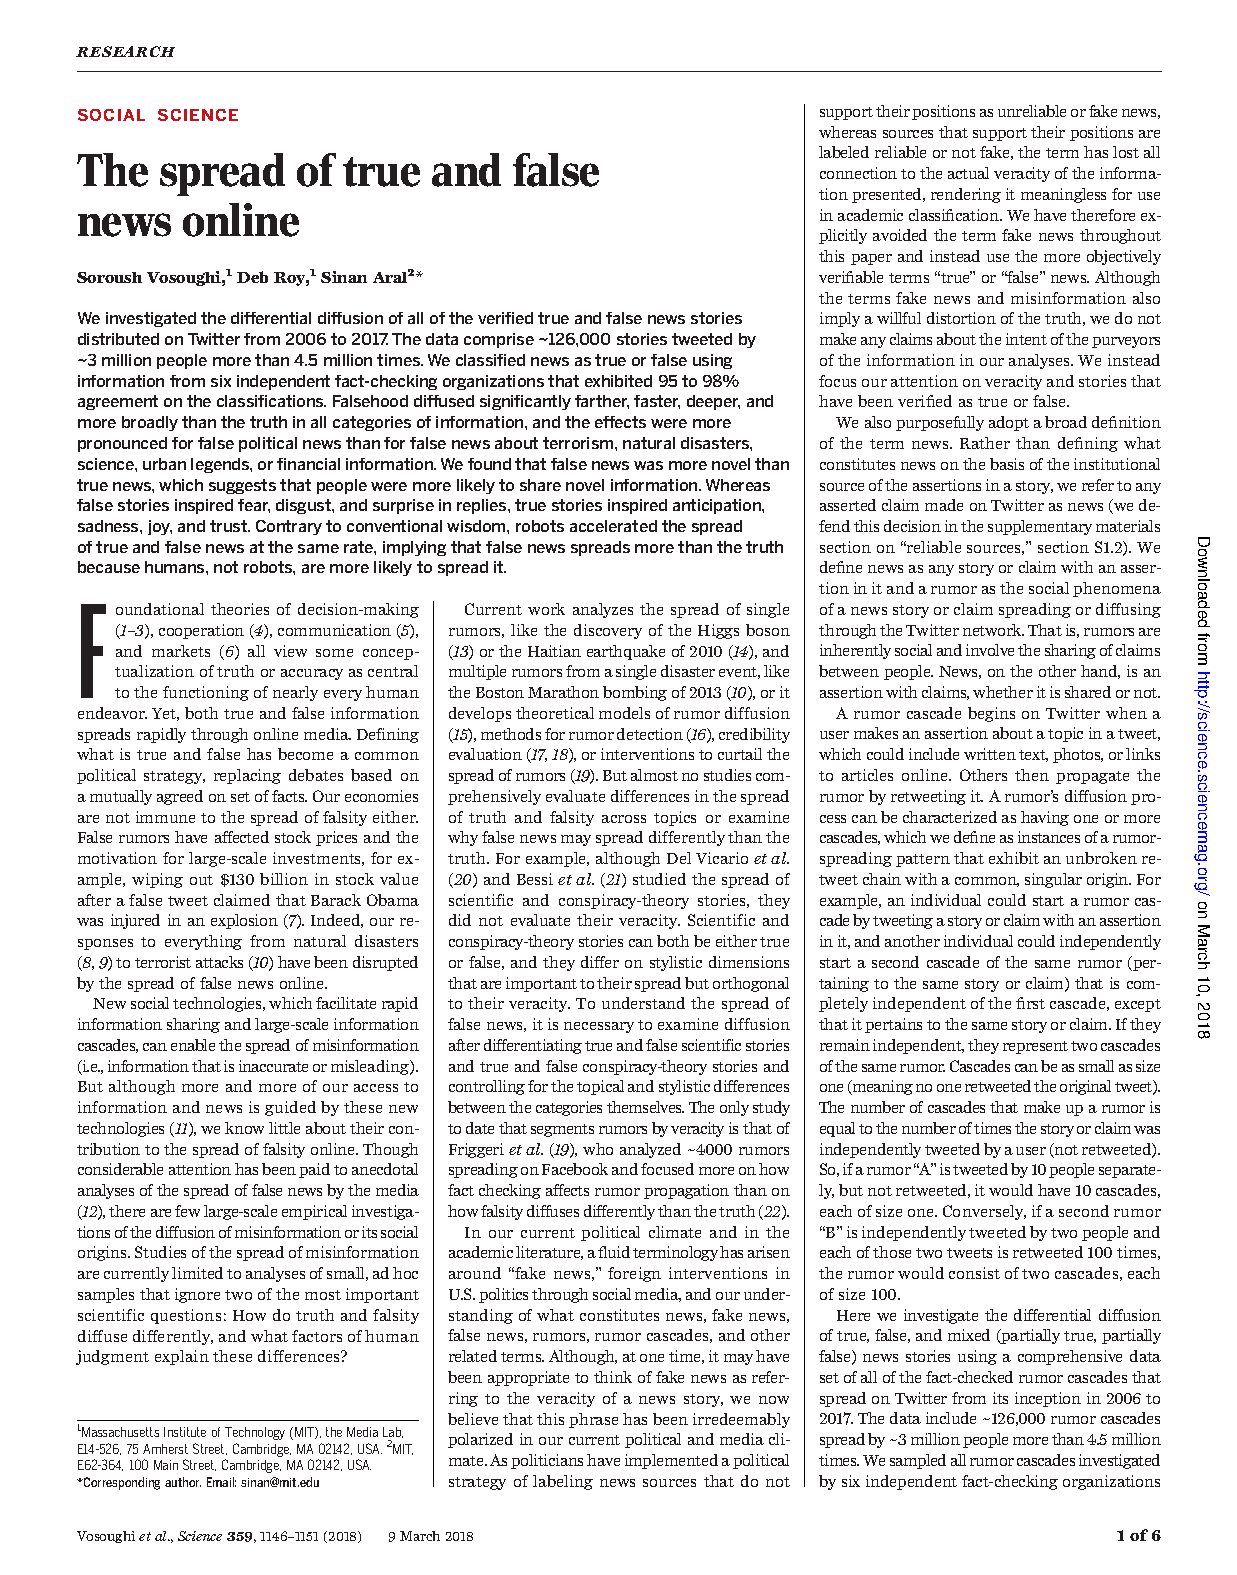
\includepdf[pages=1, scale=0.95, pagecommand=\heiti\sanhao{外\quad{}文\quad{}原\quad{}文}]{docs/translation.pdf}
% 原文剩余部分
%\end{center}


% Translation
%\setcounter{chapter}{0}
%\renewcommand{\thefigure}{~外\arabic{chapter}-\arabic{figure}~}
%\renewcommand{\theequation}{~外\arabic{chapter}-\arabic{equation}~}
%\renewcommand{\thetable}{~外\arabic{chapter}-\arabic{table}~}
%\begin{center}
%\translationtitlefont{外\quad{}文\quad{}译\quad{}文}
%\end{center}
%\vspace{8mm}
%\thispagestyle{empty}


%\end{nopagenumber}


% 开题报告
%\blankmatter
%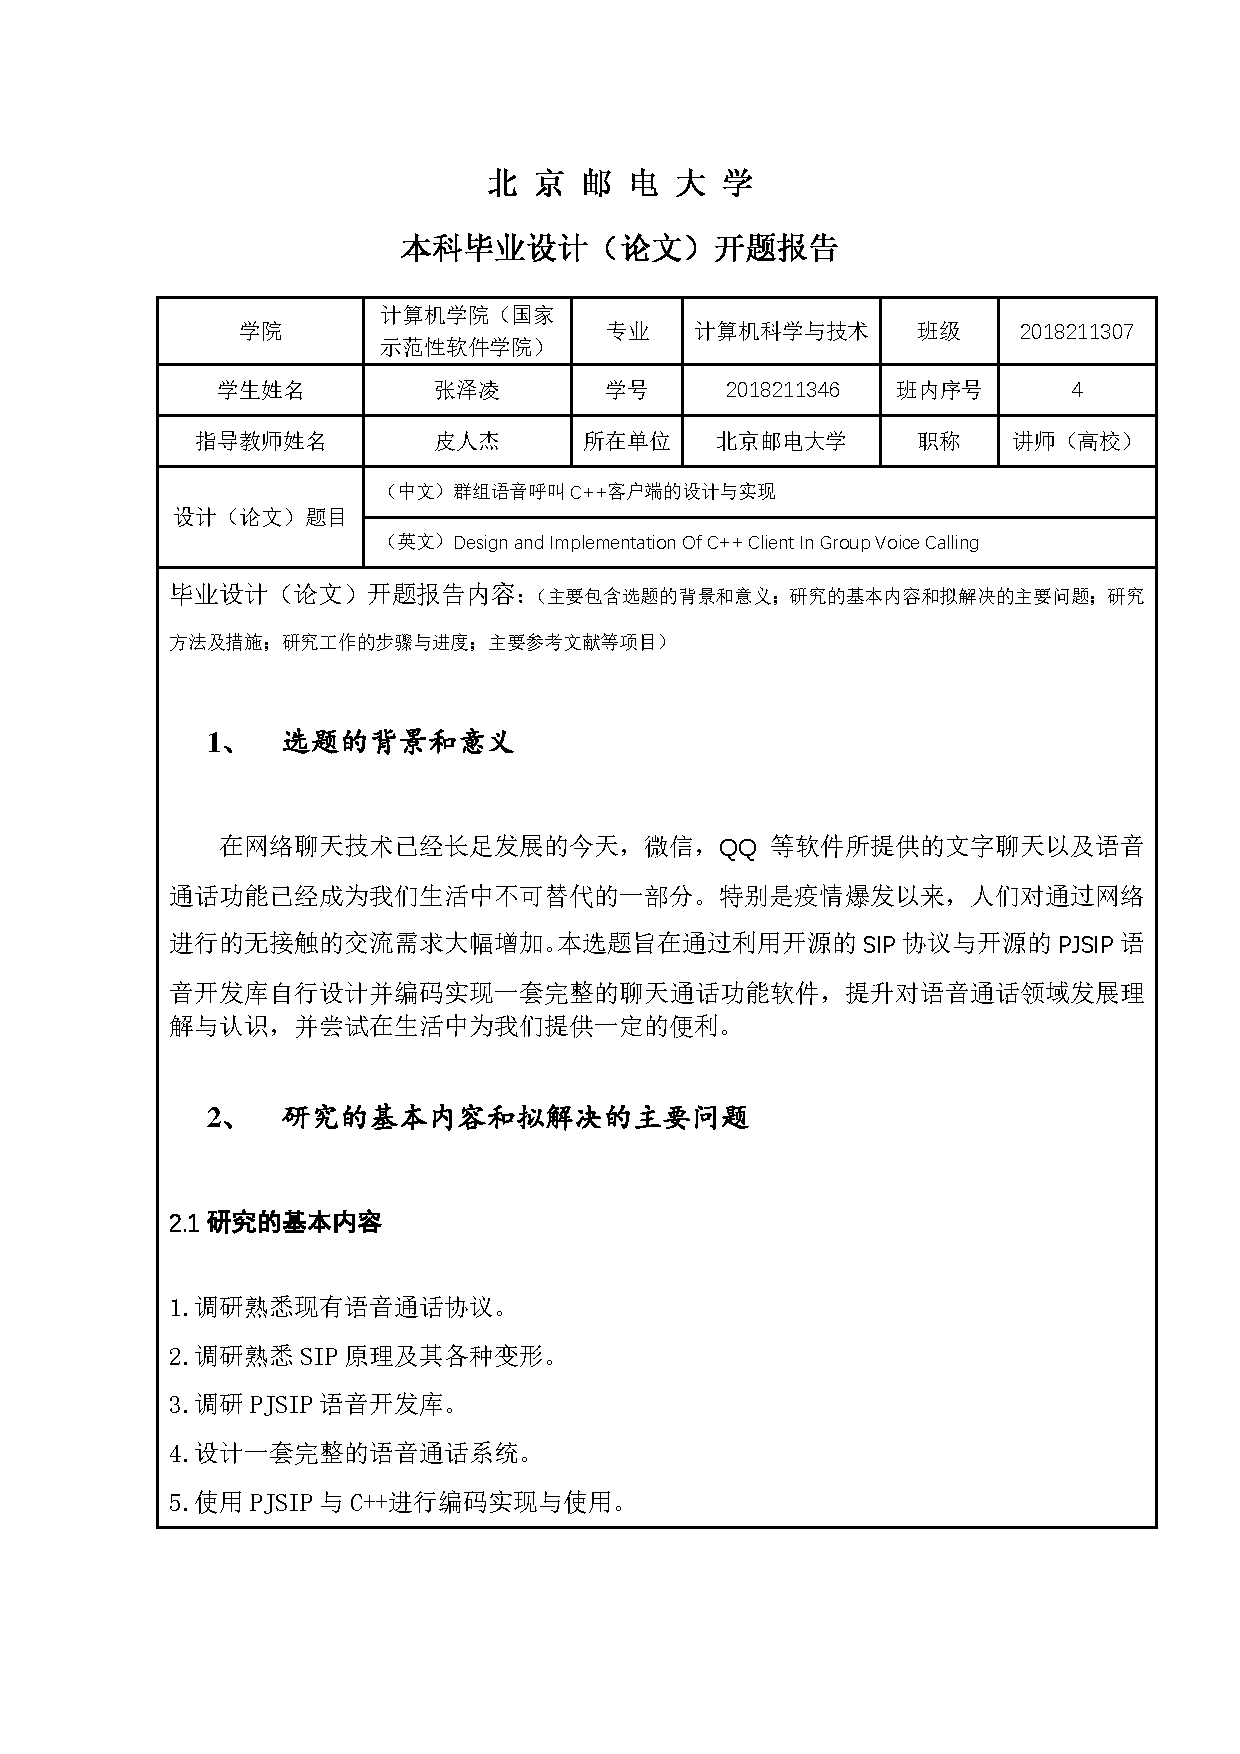
\includepdf[pages=-]{docs/openingReport.pdf} 


% 中期检查表
%\blankmatter
%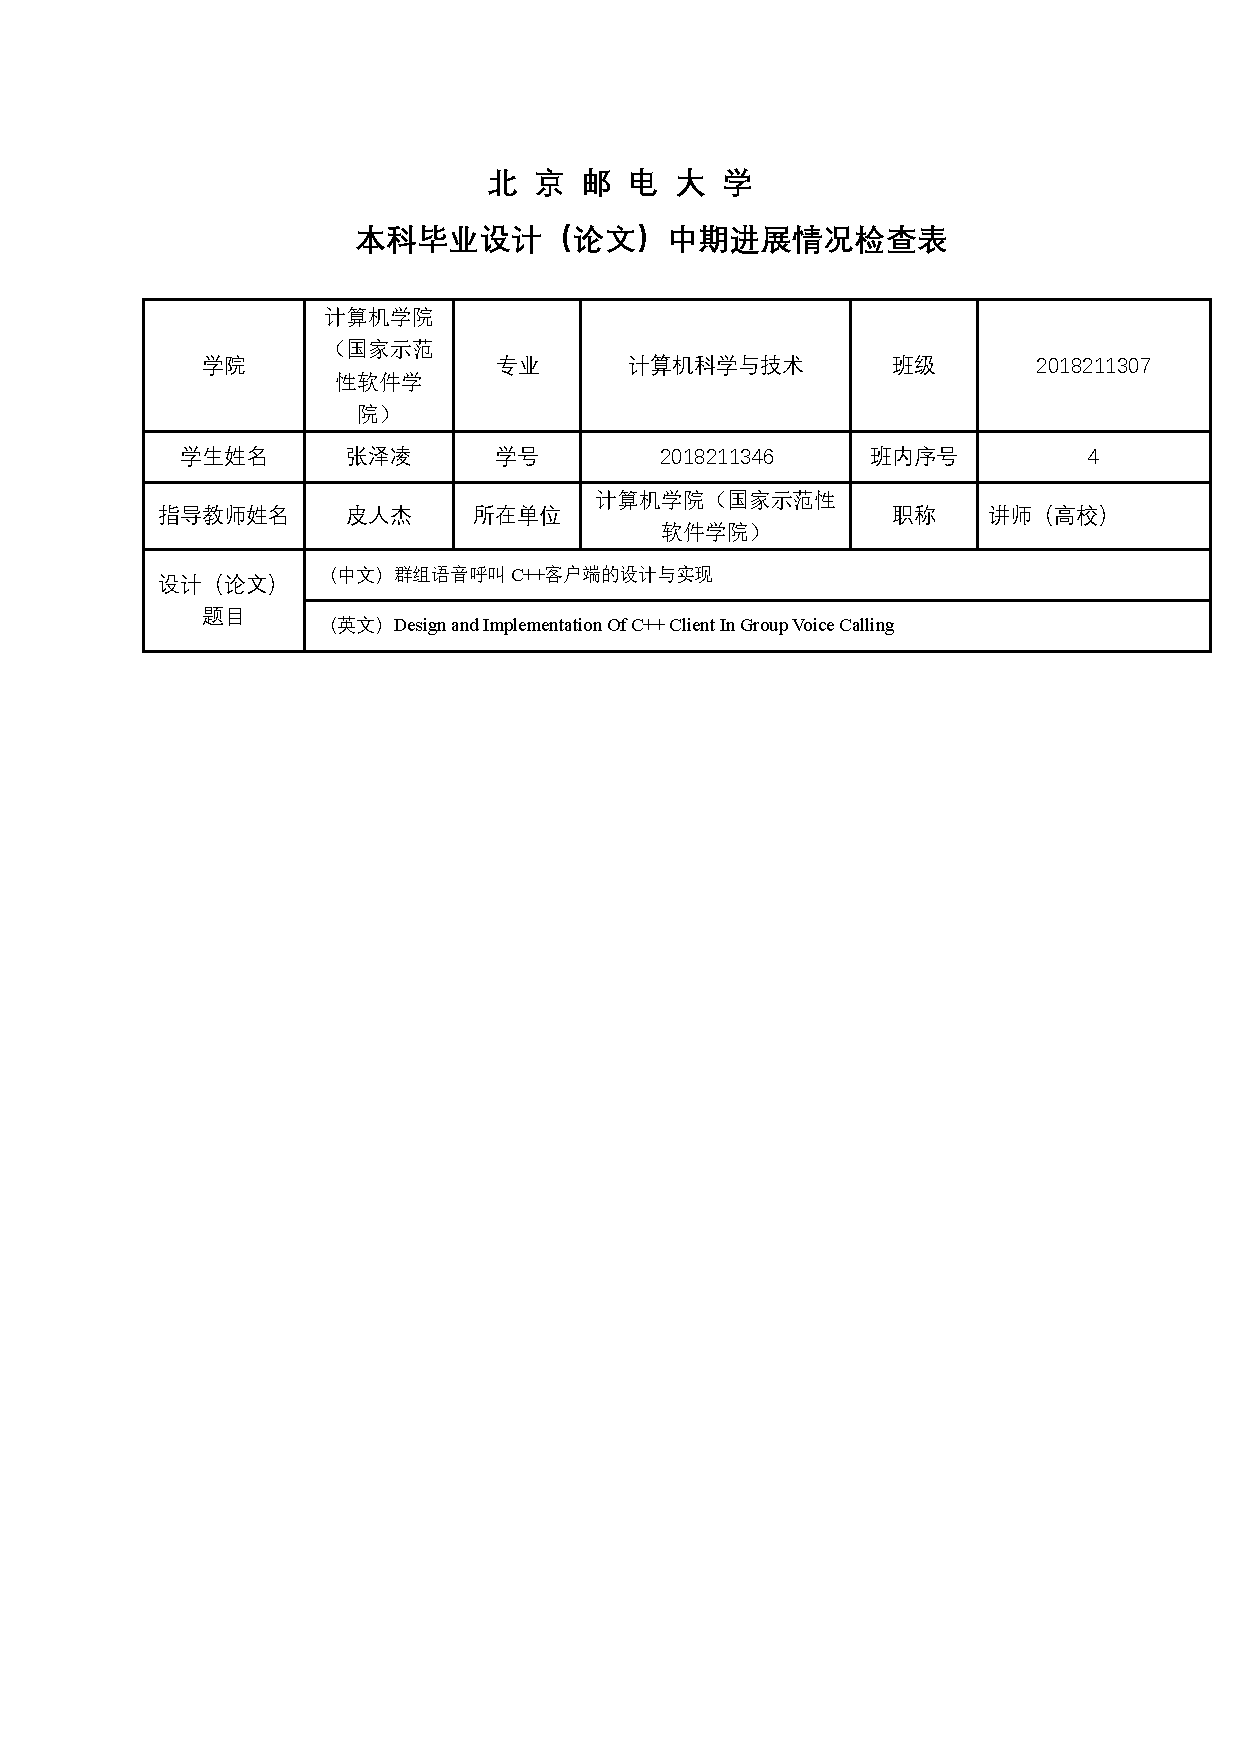
\includepdf[pages=-]{docs/interimReport.pdf} 


\end{document}
